\chapter{Overview of the Studies}
\label{ch:studies}
\chaptertoc

This chapter introduces the five studies that constitute this thesis and explains how they address the research objectives. It first maps the studies to the objectives, then summarizes what each study built, its benchmark scope, its main baselines, and its principal individual findings.

\section{Relationship Between Objectives and Studies}
\label{sec:objectives-studies}

The objectives are addressed across complementary studies rather than by a single experimental design applied identically to both recovery and mapping. Figure~\ref{fig:objective_map} maps each of the five studies to the objectives it addresses, distinguishing studies that directly address an objective's research questions from studies that partially inform it through a contrasting result or an earlier comparison with a narrower scope.

\begin{figure*}[t]
    \centering
    \resizebox{1\textwidth}{!}{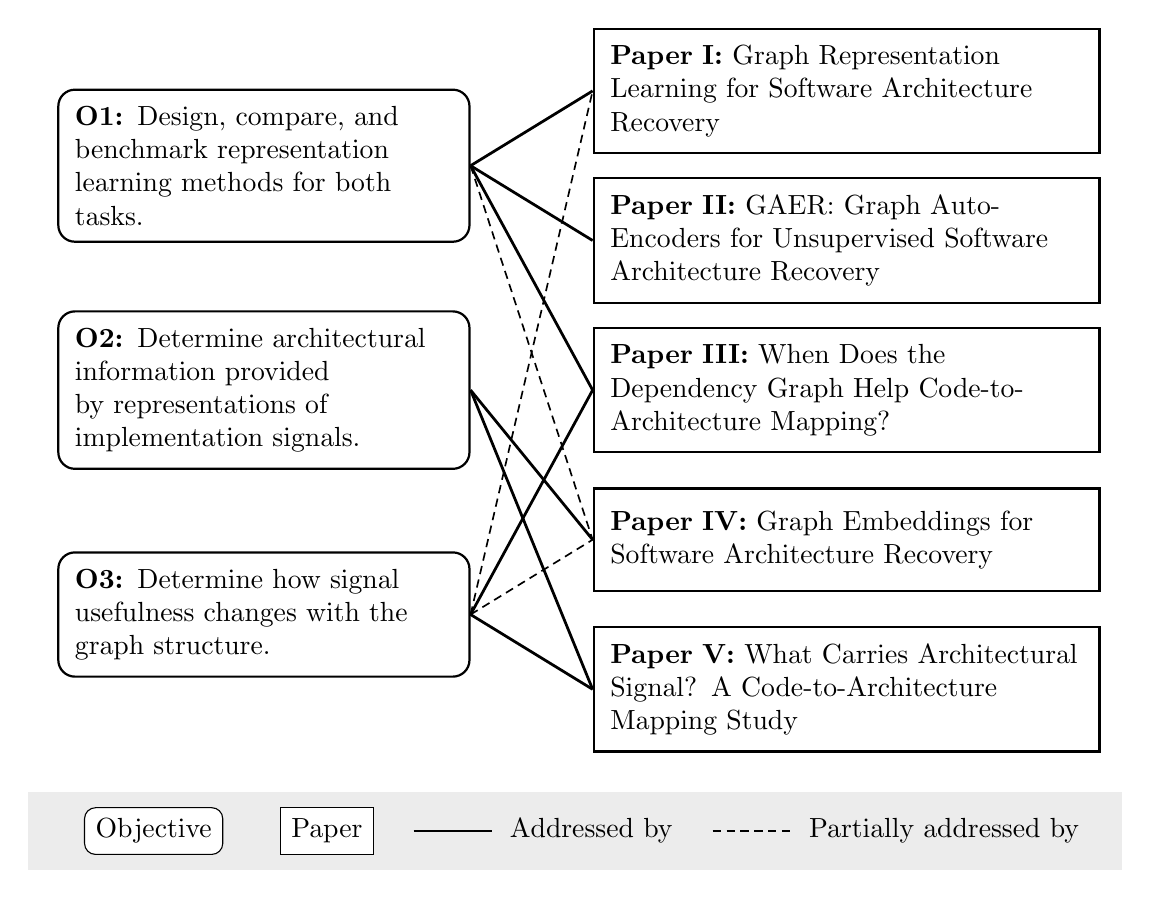
\begin{tikzpicture}[
    every node/.append style={execute at begin node={\sloppy\hyphenpenalty=10000\relax}},
    obj/.style={draw, rounded corners=6pt, line width=0.8pt, text width=4.8cm, align=left, inner sep=6pt, font=\figurefont\normalsize},
    pap/.style={draw, line width=0.8pt, text width=6cm, align=left, inner sep=6pt, minimum height=1.3cm, font=\figurefont\normalsize},
    full/.style={line width=1.0pt},
    part/.style={line width=0.6pt, dash pattern=on 3pt off 2pt}
]

% Papers
\node[pap] (P1) at (7.4, 0)     {\textbf{Paper I:} Graph Representation Learning for Software Architecture Recovery};
\node[pap] (P2) at (7.4,-1.90)  {\textbf{Paper II:} GAER: Graph Auto-Encoders for Unsupervised Software Architecture Recovery};
\node[pap] (P3) at (7.4,-3.80)   {\textbf{Paper III:} When Does the Dependency Graph Help Code-to-Architecture Mapping?};
\node[pap] (P4) at (7.4,-5.70)  {\textbf{Paper IV:} Graph Embeddings for Software Architecture Recovery};
\node[pap] (P5) at (7.4,-7.60)   {\textbf{Paper V:} What Carries Architectural Signal? A Code-to-Architecture Mapping Study};

% Objectives
\node[obj] (O1) at (0, -0.95) {\textbf{O1:} Design, compare, and benchmark representation learning methods for both tasks.};
\node[obj] (O2) at (0,-3.80)   {\textbf{O2:} Determine architectural information provided by representations of implementation signals.};
\node[obj] (O3) at (0,-6.65) {\textbf{O3:} Determine how signal usefulness changes with the graph structure.};

% Addressed by
\draw[full] (O1.east) -- (P1.west);
\draw[full] (O1.east) -- (P2.west);
\draw[full] (O1.east) -- (P3.west);
\draw[full] (O2.east) -- (P4.west);
\draw[full] (O2.east) -- (P5.west);
\draw[full] (O3.east) -- (P3.west);
\draw[full] (O3.east) -- (P5.west);

% Partially addressed by
\draw[part] (O1.east) -- (P4.west);
\draw[part] (O3.east) -- (P1.west);
\draw[part] (O3.east) -- (P4.west);

% Legend
\fill[gray!15] (-3.0,-8.9) rectangle (10.9,-9.9);
\node[draw, rounded corners=4pt, font=\figurefont\normalsize, inner sep=4pt, fill=white] at (-1.4,-9.4) {Objective};
\node[draw, font=\figurefont\normalsize, inner sep=4pt, fill=white] at (0.8,-9.4) {Paper};
\draw[full] (1.9,-9.4) -- (2.9,-9.4);
\node[font=\figurefont\normalsize, anchor=west] at (3.0,-9.4) {Addressed by};
\draw[part] (5.7,-9.4) -- (6.7,-9.4);
\node[font=\figurefont\normalsize, anchor=west] at (6.8,-9.4) {Partially addressed by};
\end{tikzpicture}}
    \caption[A high-level overview of objectives mapped to the papers.]{Mapping of research objectives to the five studies. Solid lines indicate direct coverage of the research questions; dashed lines indicate partial coverage through contrasting results or narrower comparisons.\label{fig:objective_map}}
\end{figure*}

\section{Overview of the Included Studies \label{sec:studies-overview}}
The studies progress from relation-aware graph representation learning for architecture recovery to dependency-based message passing for C2A mapping, then examine structure-only recovery and systematically compare and combine implementation signals for mapping.

\phantomsection
\subsection*{Paper~I. ~Contrastive Learning for Architecture Recovery}
\label{sec:overview-arl}

The first study~\cite{arl_2026} establishes the initial feasibility of learning architectural representations from a multi-relational software dependency graph for architecture recovery. Each dependency type is modeled as a separate directed relation among source-code files, while node features combine folder-hierarchy tokens with code identifiers not involved in inter-file dependencies. Relation-specific GAT encoders produce file representations that are trained without architectural labels using a contrastive objective and subsequently clustered to recover modules. The study also examines whether member-level interaction attributes add architectural information beyond the presence of a dependency.

The study evaluates the proposed approach on four systems against SARIF~\cite{sarif}, a hand-tuned information-fusion baseline that combines dependency, textual, and directory signals through manually designed similarity functions. The proposed approach outperforms SARIF on all four systems.

\phantomsection
\subsection*{Paper~II. GAER: Graph Auto-Encoders for Architecture Recovery}
\label{sec:overview-gaer}

The second study~\cite{gaer} extends the investigation of Paper~I to a reconstruction-based learning approach and a broader empirical setting. GAER retains the multi-relational dependency graph but replaces contrastive learning with a graph autoencoder trained to reconstruct observed dependencies. Code identifiers are now embedded with Word2Vec rather than encoded as binary vectors, while directory tokens remain binary-encoded. The study compares GCN and GAT encoders before clustering the learned representations into architectural modules.

The study evaluates ten benchmark systems against eight established dependency-based, semantic, structural representation learning, and hybrid recovery approaches. GAER achieves higher or comparable ground-truth alignment across most systems for MoJoFM, A2A, \cc{}, and ARI.

\phantomsection
\subsection*{Paper~III. When Does the Dependency Graph Help C2A Mapping?}
\label{sec:overview-c2a}

The third study~\cite{c2a_mapping} is an extended version of our previous mapping paper~\cite{jabeen2025graph}. It shifts from unsupervised architecture recovery to C2A mapping, in which the target modules are known, and a limited set of files is initially labeled. It reuses the graph construction and node features of Paper~II, expanding the labeled set into a full mapping via iterative self-training. The study compares GCN and GAT models with a graph-free MLP that uses the same file features, classifier, and self-training procedure. It further examines the effect of preserving dependency types, message-passing depth, and aggregation direction.

Across ten benchmark systems, all learned approaches outperform the Naive Bayes mapping baseline~\cite{olsson2022automatically}.

\phantomsection
\subsection*{Paper~IV. Graph Embeddings for Architecture Recovery}
\label{sec:overview-structsar}

The fourth study returns to architecture recovery but isolates the value of structural and organizational information by removing lexical file features~\cite{structsar}. Unlike the first three studies, it learns representations from graph structure alone. The study first evaluates recovery from a homogeneous dependency graph using Node2Vec, a GAT encoder trained within a variational graph autoencoder, and the same encoder applied to a graph rewired by PPR diffusion (GAT-DC). It then extends the graph with folder nodes and containment relations, comparing the dependency structure alone against the dependency structure combined with developer-defined folder organization, using MetaPath2Vec, a heterogeneous GAT (HGAT), and a variant that preserves dependency types rather than merging them (HGAT-TD).

The study evaluates eleven systems against four classical dependency-only recovery baselines. The dependency-only GAT, GAT-DC, and Node2Vec outperform these baselines on most systems and metrics.

\phantomsection
\subsection*{Paper~V. What Carries Architectural Signal? A C2A Mapping Study}
\label{sec:overview-hetmap}

The fifth study examines which implementation signals contribute to C2A mapping and how their usefulness changes with graph structure and message passing~\cite{hetmap}. It compares structural Node2Vec, lexical Word2Vec, and contextual UniXcoder file representations, with UniXcoder evaluated before and after dependency-guided contrastive fine-tuning. Each representation is first evaluated using a graph-free MLP. Node2Vec, Word2Vec, and fine-tuned UniXcoder then initialize HGT on four graph configurations: files only, files with folders, files with members, and the full folder-file-member graph, with dependencies merged into a single relation type. Each member node summarizes the program members of one file. A GAT on the file-level dependency graph is evaluated as a second message-passing predictor.

The study uses the ten systems and labeled sets of Paper~III. The MLP is the baseline for the graph configurations, and a directory-hierarchy rule is the reference for folder-augmented configurations. The rule assigns an unlabeled file the most common module among the labeled files in its directory, backing off to progressively larger enclosing subtrees when the directory has no labeled file.
